\usetikzlibrary{positioning}

\usetikzlibrary{arrows}
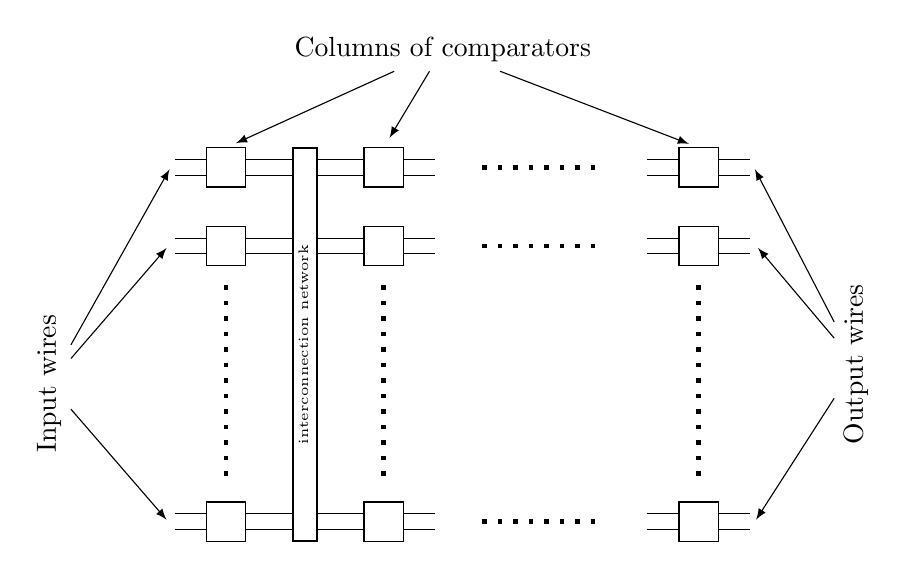
\begin{tikzpicture}

\draw  (-5,4.5) rectangle (-4.5,4);
\draw  (-5,3.5) rectangle (-4.5,3);
\draw  (-5,0) rectangle (-4.5,-0.5);

\draw[thick] (-3.9,4.5) rectangle (-3.6,-0.5);

\node[rotate=90] at (-3.77,2) {\tiny interconnection network};

\draw  (-3,4.5) rectangle (-2.5,4);
\draw  (-3,3.5) rectangle (-2.5,3);
\draw  (-3,0) rectangle (-2.5,-0.5);
\draw  (1,4.5) rectangle (1.5,4);
\draw  (1,3.5) rectangle (1.5,3);
\draw  (1,0) rectangle (1.5,-0.5);

\draw  (-4.5,4.35) rectangle (-3.9,4.15);
\draw  (-4.5,3.35) rectangle (-3.9,3.15);

\draw  (-3.6,4.35) rectangle (-3,4.15);
\draw  (-3.6,3.35) rectangle (-3,3.15);

\draw  (-4.5,-0.15) rectangle (-3.9,-0.35);
	\draw  (-3.6,-0.15) rectangle (-3,-0.35);

%% dots 
\draw[loosely dotted, ultra thick] (-1.5,4.25) -- (0,4.25);
\draw[loosely dotted, ultra thick] (-1.5,3.25) -- (0,3.25);
\draw[loosely dotted, ultra thick] (-1.5,-0.25) -- (0,-0.25);

\draw[loosely dotted, ultra thick] (-4.75,2.75) -- (-4.75,0.25);
\draw[loosely dotted, ultra thick] (-2.75,2.75) -- (-2.75,0.25);
\draw[loosely dotted, ultra thick] (1.25,2.75) -- (1.25,0.25);

%% wires
\draw (-5.4,4.35) node (v2) {} -- (-5,4.35);
\draw (-5.4,4.15) -- (-5,4.15);
\draw (-5.4,3.35) node (v3) {} -- (-5,3.35);
\draw (-5.4,3.15) -- (-5,3.15);
\draw (-5.4,-0.35) node (v4) {} -- (-5,-0.35);
\draw (-5.4,-0.15) -- (-5,-0.15);

\begin{scope}[shift={(2.9,0)}]
\draw (-5.4,4.35) -- (-5,4.35);
\draw (-5.4,4.15) -- (-5,4.15);
\draw (-5.4,3.35) -- (-5,3.35);
\draw (-5.4,3.15) -- (-5,3.15);
\draw (-5.4,-0.35) -- (-5,-0.35);
\draw (-5.4,-0.15) -- (-5,-0.15);
\end{scope}

\begin{scope}[shift={(6,0)}]
\draw (-5.4,4.35) -- (-5,4.35);
\draw (-5.4,4.15) -- (-5,4.15);
\draw (-5.4,3.35) -- (-5,3.35);
\draw (-5.4,3.15) -- (-5,3.15);
\draw (-5.4,-0.35) -- (-5,-0.35);
\draw (-5.4,-0.15) -- (-5,-0.15);
\end{scope}

\begin{scope}[shift={(6.9,0)}]
\draw (-5.4,4.35) -- (-5,4.35) node (v8) {};
\draw (-5.4,4.15) -- (-5,4.15);
\draw (-5.4,3.35) -- (-5,3.35) node (v7) {};
\draw (-5.4,3.15) -- (-5,3.15);
\draw (-5.4,-0.35) -- (-5,-0.35) node (v6) {};
\draw (-5.4,-0.15) -- (-5,-0.15);
\end{scope}

% labels

\node[rotate=90] (v1) at (-7,1.5) {Input wires};

\node[rotate=90] (v5) at (3.25,1.75) {Output wires};
\draw [-latex] (v1) edge (v2);
\draw [-latex] (v1) edge (v3);
\draw [-latex] (v1) edge (v4);
\draw [-latex] (v5) edge (v6);
\draw [-latex] (v5) edge (v7);
\draw [-latex] (v5) edge (v8);

\node (v9) at (-2,5.75) {Columns of comparators};
\node (v10) at (-4.75,4.5) {};
\node (v11) at (-2.75,4.5) {};
\node (v12) at (1.25,4.5) {};
\draw [-latex] (v9) edge (v10);
\draw [-latex] (v9) edge (v11);
\draw [-latex] (v9) edge (v12);
\end{tikzpicture}